%  Copyright 2020-2024 Robert Bosch GmbH
%
%  Licensed under the Apache License, Version 2.0 (the "License");
%  you may not use this file except in compliance with the License.
%  You may obtain a copy of the License at
%
%      http://www.apache.org/licenses/LICENSE-2.0
%
%  Unless required by applicable law or agreed to in writing, software
%  distributed under the License is distributed on an "AS IS" BASIS,
%  WITHOUT WARRANTIES OR CONDITIONS OF ANY KIND, either express or implied.
%  See the License for the specific language governing permissions and
%  limitations under the License.

\chapter{Installation and start}

The \textbf{RobotFramework AIO} can be installed under Windows and under Linux in this way:

\begin{itemize}
   \item \textbf{Win10}

         Double-click the \plog{setup\_.*.exe} file and follow the instructions.

   \item \textbf{Linux}

         If already installed, remove the previous version (this will not remove your own data):

         \begin{pythonlog}
sudo apt-get remove robotframework-aio
\end{pythonlog}

         Install/Update now the current version (assumed you are in the download directory):
         \begin{pythonlog}
sudo apt-get install ./setup_RobotFramework_AIO_OSD6Linux\_*.deb
\end{pythonlog}

\end{itemize}

After the installation is finished, a new \textbf{VSCodium} icon is present on desktop:
\begin{itemize}
   \item \textbf{Win10}

         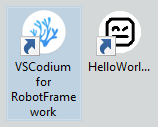
\includegraphics[scale=0.7]{./include/graphics/installation/Icon_Win10.png}
         (together with a link to the example robot file \plog{HelloWorld.robot})

   \item \textbf{Linux}

         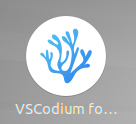
\includegraphics[scale=0.7]{./include/graphics/installation/Icon_Linux.png}
\end{itemize}

A double-click starts the application.

\newpage

On first start the \textbf{VSCodium} main window appears like this:

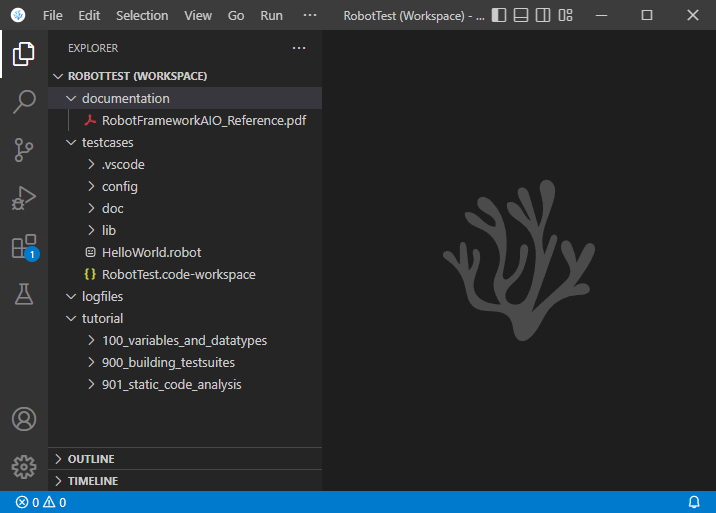
\includegraphics[scale=0.8]{./include/graphics/installation/MainWindow.png}

The preconfigured workspace contains the following parts:

\begin{itemize}
   \item The main documentation \plog{RobotFrameworkAIO_Reference.pdf} (including the documentation of all components that are part of the \textbf{RobotFramework AIO})
   \item A \plog{testcases} folder containing (beneath other elements) the  example robot file \plog{HelloWorld.robot}
   \item A \plog{logfiles} folder in which all log files and reports will be placed (from tests that are executed with \textbf{VSCodium})
   \item A \plog{tutorial} folder containing a large bunch of testfiles that can be used for self-dependent learning
\end{itemize}

\newpage

For the usage of the predefined infrastructure (e.g. the \plog{logfiles} folder), the \textbf{VSCodium} provides an adapted configuration of the \textbf{Run} button.
This button executes the robot file selected in project explorer of \textbf{VSCodium}.

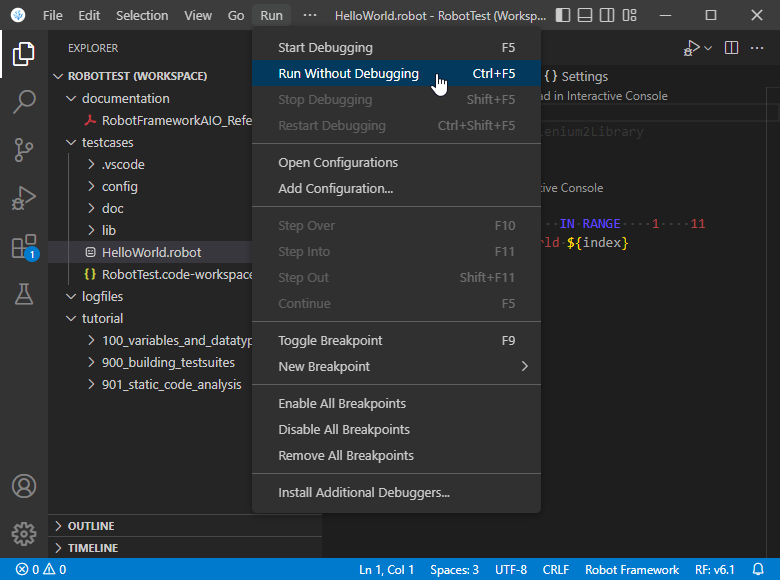
\includegraphics[scale=0.7]{./include/graphics/installation/RunButton.png}

After test execution, the links to log files and reports can be found in the \textbf{TERMINAL} window.

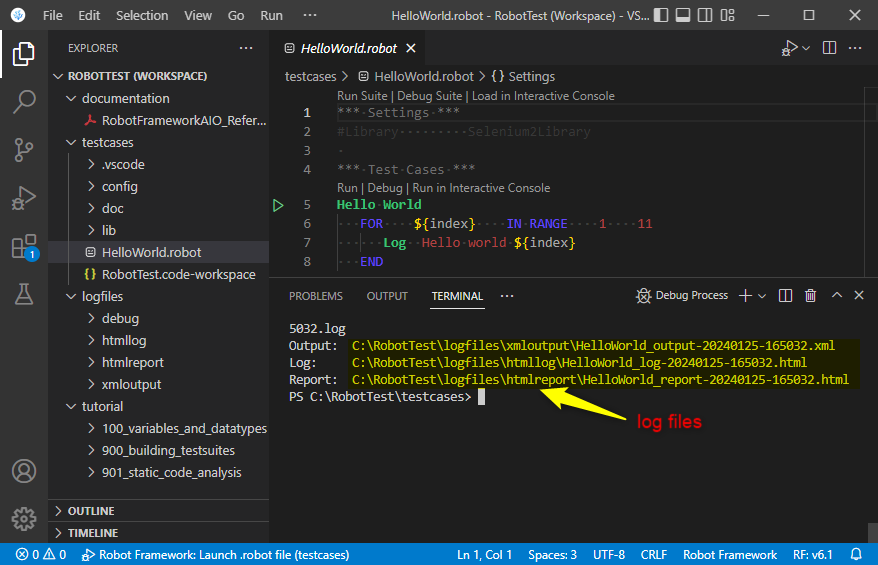
\includegraphics[scale=0.7]{./include/graphics/installation/TestResults.png}

Every file there can be opened by CTRL+click on the selected file.


